
Bài toán tối ưu hóa là bài toán cực đại hóa hoặc cực tiểu hóa một giá trị thực của hàm nhiều biến được gọi là hàm chi phí. Nếu bài toán là cực đại hóa hàm chi phí $f$ thì chỉ cần cực tiểu hóa $-f$ là đủ. Do đó, không mất tính tổng quát khi chỉ xem xét việc cực tiểu hóa.

Các bài toán tối ưu hóa được phân loại một cách tương đối thành hai loại, dễ và khó. Nói một cách đơn giản hơn, các bài toán dễ là những bài toán mà chúng ta có thuật toán để giải theo đa thức bước trong kích thước hệ thống (độ phức tạp đa thức). Ngược lại, đối với các bài toán khó, tất cả các thuật toán đã biết đều phải thực hiện rất nhiều bước theo cấp số nhân để đạt được lời giải chính xác (độ phức tạp theo cấp số nhân). Đối với những bài toán này, hầu như không thể tìm ra lời giải chính xác nếu kích thước bài toán vượt quá một giá trị vừa phải.

Trong khóa luận hiện tại, chúng ta sẽ thảo luận về các thuật toán tổng quát là ủ mô phỏng (Simulated Annealing) và ủ lượng tử (Quantum Annealing).

Trong SA, hàm chi phí cần giảm thiểu được xác định bằng năng lượng của hệ thống cơ học thống kê. Sau đó, hệ thống được cung cấp nhiệt độ, một tham số điều khiển được đưa vào một cách giả tạo, bằng cách giảm từ từ từ giá trị cao xuống 0, chúng ta hy vọng sẽ đưa hệ thống về trạng thái có giá trị năng lượng thấp nhất, đạt được lời giải của bài toán tối ưu hóa.

Trong các ứng dụng thực tế, SA rất phổ biến do khả năng áp dụng tổng quát, hiệu suất hợp lý và việc triển khai tương đối dễ dàng trong hầu hết các trường hợp. SA thường được sử dụng như một phương pháp để thu được nghiệm gần đúng trong thời gian tính toán hữu hạn vì nó cần một thời gian dài vô hạn để đạt được nghiệm chính xác bằng cách giữ hệ thống gần với trạng thái cân bằng nhiệt.

Trong SA, chúng ta sử dụng các dao động nhiệt (cổ điển) để cho phép hệ thống chuyển từ trạng thái này sang trạng thái khác vượt qua các rào cản năng lượng trung gian để tìm kiếm trạng thái năng lượng thấp nhất mong muốn.

Trong QA, chúng ta khéo léo kiểm soát cường độ của những dao động lượng tử này để hệ thống cuối cùng đạt đến trạng thái cơ bản, giống như SA, trong đó chúng ta giảm nhiệt độ từ từ và đường hầm lượng tử giữa các trạng thái cổ điển khác nhau thay thế bước nhảy nhiệt trong SA (Hình~\ref{fig:quantum_tunneling_and_hill_climbing}).

\begin{figure}[h]
	\centering
	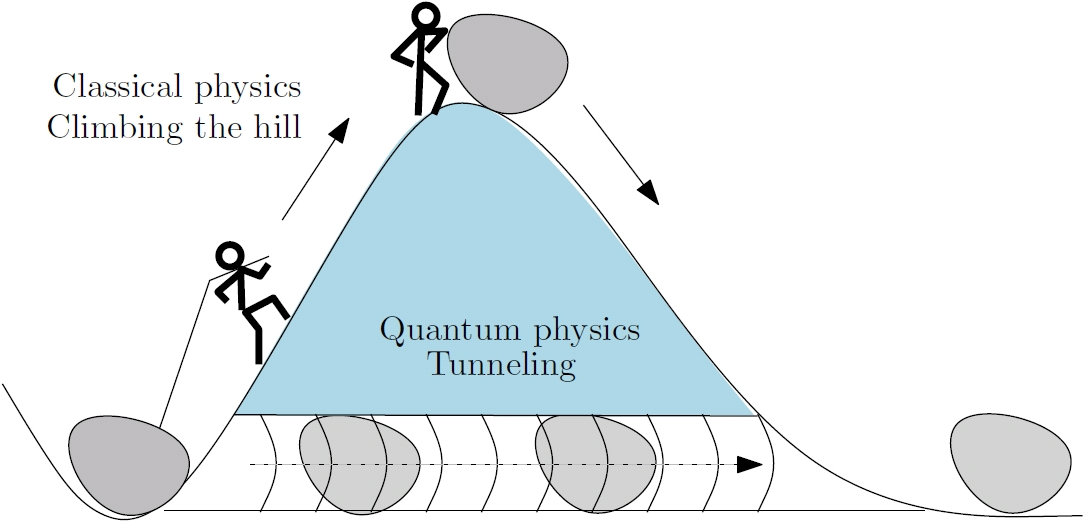
\includegraphics[width=0.7\textwidth]{images/quantum tunneling.png}
	\caption{Đường hầm lượng tử (trong QA) và bước nhảy nhiệt(leo đồi)(trong SA) \cite{Quantum tunneling}}
	\label{fig:quantum_tunneling_and_hill_climbing}
\end{figure}

Ý tưởng vật lý đằng sau quy trình như vậy là giữ cho hệ thống ở gần trạng thái cơ bản tức thời của hệ lượng tử, tương tự như trạng thái gần như cân bằng được giữ trong quá trình tiến hóa theo thời gian của SA. Tương tự như SA, về nguyên tắc, QA là một thuật toán tổng quát có thể áp dụng cho bất kỳ bài toán tối ưu hóa tổ hợp nào và được sử dụng như một phương pháp để đạt được lời giải gần đúng trong một khoảng thời gian hữu hạn nhất định.

%Người đọc có thể thắc mắc tại sao người ta lại phải phát minh ra một thuật toán tổng quát khác khi chúng ta đã có SA mạnh mẽ. Câu trả lời ngắn gọn là QA tốt hơn SA trong hầu hết các trường hợp, ít nhất là về mặt lý thuyết. Các kết quả phân tích và số học chỉ ra rằng thời gian tính toán cần thiết để đạt được độ chính xác nhất định của câu trả lời trong QA ngắn hơn so với SA. Ngoài ra, mức độ lỗi đối với QA nhỏ hơn SA nếu chúng ta chạy thuật toán trong một khoảng thời gian hữu hạn cố định.

%Một hạn chế của QA là việc triển khai thực tế đầy đủ phải dựa vào máy tính lượng tử vì chúng ta cần giải phương trình Schr¨odinger phụ thuộc thời gian ở quy mô rất lớn.


\section{Lý do chọn đề tài}
\subsection{Lý do chọn bài toán xếp hậu}


Bài toán xếp hậu là một bài toán kinh điển về bài toán NP-đầy đủ, được biết đến với tính chất thách thức của nó. Trong lĩnh vực tối ưu hóa và trí tuệ nhân tạo, nó có vai trò quan trọng trong nghiên cứu học thuật và ứng dụng thực tiễn như lý thuyết đồ thị, thiết kế mạch, điều khiển không lưu
, nén dữ liệu và lập lịch tác vụ máy tính \cite{A survey of known results and research areas for}. 
% Có thể nêu nhiều hơn ứng dụng hoặc chi tiết, cụ thể

\subsection{Lý do chọn ủ lượng tử}

Điện toán lượng tử (Quantum Computing) là một lĩnh vực nghiên cứu đang phát triển nhanh chóng, hứa hẹn một mô hình mới để giải quyết các bài toán tính toán đầy thách thức. Nó được giới thiệu lần đầu tiên vào đầu những năm 1980 bởi nhà vật lý Paul Benioff
\cite{The computer as a physical system}
và độc lập bởi Richard Feynman
\cite{Simulating physics with computers}.
Những đề xuất ban đầu này của điện toán lượng tử đề cập đến việc sử dụng các tính chất cơ bản của lượng tử như sự chồng chất (quantum superposition) và sự vướng víu (quantum entanglement) để thực hiện tính toán và mô phỏng tự nhiên. Trong những thập kỷ kể từ đó, những tiến bộ đáng kể của cả thuật toán và phần cứng đã mở rộng tiềm năng và phạm vi sử dụng của máy tính lượng tử. Các công trình chuyên đề của Deutsch 
\cite{Quantum computational networks}
và Grover 
\cite{A Fast Quantum Mechanical Algorithm for Database Search}
đã chỉ ra rằng các thuật toán lượng tử có thể mang lại sự tăng tốc tiệm cận (tăng tốc không đổi trong giới hạn kích thước hệ thống lớn) so với các lời giải cổ điển của chúng.
% đối  tác cổ điển??
Trong một số trường hợp, điều này thậm chí có thể dẫn đến các thuật toán nhanh hơn theo cấp số nhân, chẳng hạn như 
thuật toán biến đổi lượng tử Fourier
\cite{An approximate Fourier transform useful in quantum factoring}. 


Trong đề xuất của Deutsch \cite{Quantum computational networks}, điện toán lượng tử phổ quát theo mô hình đã trở thành "tiêu chuẩn" là mô hình mạch và mô hình cổng. Trong mô hình cổng, việc tính toán được thực hiện bằng cách áp dụng một chuỗi các cổng đơn nhất cho một tập hợp các hạt lượng tử (qubit), trạng thái của chúng có thể được đo khi kết thúc tính toán 
\cite{Quantum computational networks}
. Ngược lại, trong tính toán lượng tử đoạn nhiệt (Adiabatic Quantum Computing), người ta chuẩn bị trạng thái lượng tử nhiều hạt lượng tử ban đầu làm trạng thái cơ bản của Hamiltonian đơn giản, áp dụng tiến hóa thời gian đoạn nhiệt, thay đổi hệ thống thành Hamiltonian cuối cùng có trạng thái cơ bản, mã hóa lời giải mong muốn (tối ưu hóa) bài toán. 

Bất chấp những nỗ lực đáng kể về mặt lý thuyết     \cite{Adiabatic quantum computation} và thực nghiệm     \cite{Evidence for quantum annealing with more than one hundred qubits}, việc tăng tốc lượng tử trong tính toán lượng tử đoạn nhiệt vẫn chưa được chứng minh trong một thử nghiệm nào. Do đó, việc chứng minh lợi thế lượng tử bằng cách giải quyết các bài toán tối ưu hóa bằng các công cụ mô phỏng lượng tử là một bước quan trọng hướng tới sự phát triển của các bộ tối ưu 
% (general programmable quantum optimizers ?)
hóa lượng tử có thể lập trình tổng quát     \cite{A quantum annealin architecture with all-to-all connectivity from local interactions} \cite{Minor-embedding in adiabatic quantum computation: I. the parameter setting problem}.


\section{Giới thiệu về bài toán}
\subsection{Bài toán bao phủ chính xác (Exact Cover)}

Bài toán bao phủ chính xác có thể định nghĩa như sau: \cite{Ising formulations}

\textbf{Đầu vào: } Cho một tập $U = \{1, \dots, n \}$; và các tập con $V_i \subseteq U (i = 1, \dots, N)$ thoả mãn:

$$U = \bigcup_{i=1}^{} V_i$$


\textbf{Câu hỏi:} Liệu rằng có một tập con của tập các tập {$V_i$}, được gọi là R, sao cho các phần tử của R là các tập không giao nhau và hợp của các phần tử của R là U không?

Đây là một bài toán NP-đầy đủ.\\
Hàm Hamiltonian chúng ta sử dụng là: 
\[ H_A = A \sum_{\alpha=1}^{n} \left(1 - \sum_{i:\alpha \in V_i} x_i\right)^2\]

trong đó: $\alpha$ biểu thị các phần tử của U, $i$ biểu thị những tập con $V_i$. 

$H_A$ = 0 khi mỗi phần tử được đưa vào đúng một lần, hàm ý rằng các tập là không giao nhau. Sự tồn tại trạng thái năng lượng cơ bản H = 0 tương ứng với sự tồn tại nghiệm của bài toán bao phủ chính xác.

\subsection{Bài toán xếp hậu (N-Queens)}
Bài toán tám quân hậu lần đầu tiên được đề xuất bởi Max Bezzel trên một tạp chí cờ vua ở Berlin vào năm 1848 \cite{Proposal of eight queens problem}. Bài toán ban đầu là làm thế nào để đặt tám quân hậu lên bàn cờ sao cho không có quân hậu nào tấn công quân hậu khác. Bởi vì quân hậu được phép di chuyển bất kỳ khoảng trống nào theo chiều ngang, chiều dọc hoặc đường chéo, điều này có nghĩa là không quân hậu nào có thể ở cùng hàng, cột hoặc đường chéo với bất kỳ quân hậu nào khác.

Ví dụ, hình \ref{fig:8-queens-solution} đưa ra một lời giải cho bài toán tám quân hậu.

%\begin{figure}[h]
%	\centering
%	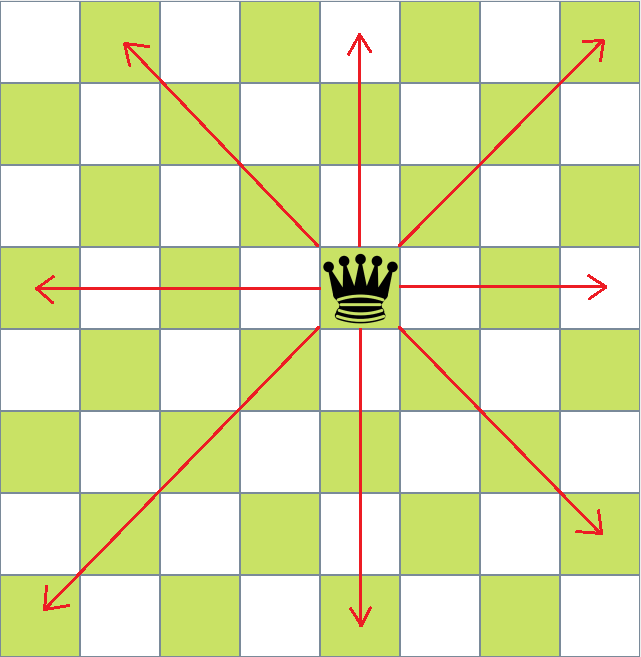
\includegraphics[width=0.5\textwidth]{images/direction-of-queen.png}
%	\caption{Các hướng đi của quân hậu}
%	\label{fig:direction-of-queen}
%	
%\end{figure}

\begin{figure}[h]
	\centering
	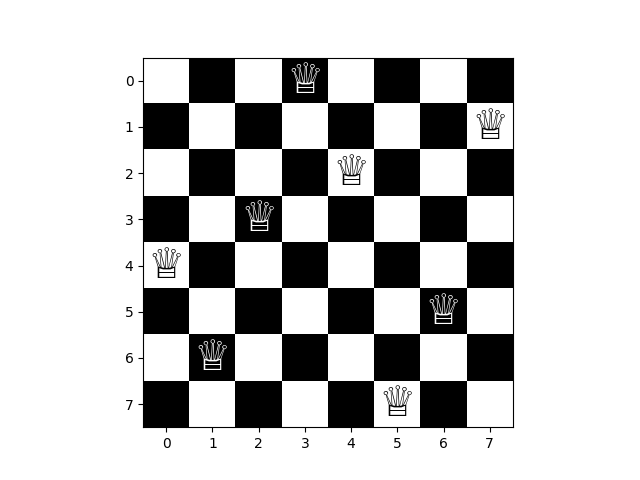
\includegraphics[width=0.7\textwidth]{images/8-queens-solution.png}
	\caption{Một lời giải cho bài toán tám quân hậu}
	\label{fig:8-queens-solution}
	
\end{figure}

Nếu số lượng quân hậu của bài toán được mở rộng, nó sẽ trở thành bài toán xếp hậu. 
Xếp hậu là một bài toán tối ưu hoá, dẫn xuất từ bài toán bao phủ chính xác. Cách tốt nhất để giải bài toán dạng này là áp dụng thuật toán vét cạn, quay lui và duyệt cây,\dots . Chúng ta tính toán tất cả các trường hợp cho tất cả các đầu vào có thể và xem xét giá trị hợp lệ . Tuy nhiên, cách tiếp cận này không phải lúc nào cũng có thể thực hiện được. Đôi khi, đầu vào số hậu không nhỏ.
May mắn thay, đó không phải là thuật toán duy nhất để giải bài toán dạng này. Có nhiều thuật toán có khả năng xác định điểm tối ưu mà không cần phải phân tích từng điểm của nó. Một trong số đó là ủ lượng tử.

\section{Ủ lượng tử}

\subsection{Nguyên lý hoạt động}
Ủ lượng tử là phiên bản lượng tử của quá trình ủ mô phỏng.
Ủ mô phỏng là một chiến lược xác suất được sử dụng để giải quyết các bài toán tối ưu hóa.

Không đi sâu vào chi tiết của thuật toán, chúng ta có thể giải thích ý tưởng đằng sau nó bằng cách nghĩ về một quả bóng lăn dọc theo đồ thị của hàm số, rơi vào các lỗ được xác định bởi cực tiểu. Mỗi khi một quả bóng rơi vào một cái lỗ, nó sẽ nhận được một lượng năng lượng nhất định, đủ để khiến nó nhảy qua một phần đồ thị khác, tìm kiếm những điểm cực tiểu sâu hơn. (Hình~\ref{fig:Quả bóng lăn dọc theo đồ thị hàm số})

\begin{figure}[h!]
    \centering
    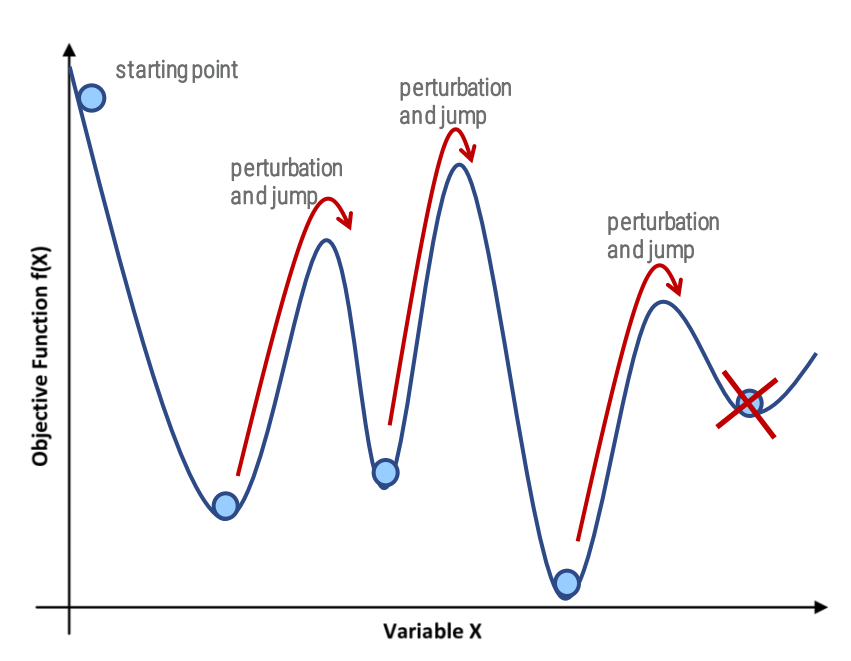
\includegraphics[width=0.7\textwidth]{images/SA.png}
     \caption{Đồ thị hàm số minh họa cho hàm mục tiêu trong ủ mô phỏng}
     \label{fig:Quả bóng lăn dọc theo đồ thị hàm số}
\end{figure}

 Về mặt trực quan, chúng ta có thể coi quá trình ủ lượng tử là một quá trình ủ mô phỏng trong đó quả bóng, một vật thể vĩ mô, được thay thế bằng một hạt cực nhỏ. 

Vậy quá trình ủ lượng tử diễn ra như thế nào? Cốt lõi của thuật toán nằm ở Định lý Đoạn nhiệt: Một hệ vật lý vẫn ở trạng thái riêng tức thời nếu một nhiễu loạn nhất định tác động lên nó đủ chậm và nếu có một khoảng cách giữa giá trị riêng và phần còn lại của phổ Hamilton.

Tối ưu hóa thông qua ủ lượng tử bắt đầu bằng việc chọn một hàm mục tiêu khác với hàm muốn tối ưu hóa. Sự lựa chọn thường rơi vào một hàm đơn giản. (Hình~\ref{fig:Đồ thị hàm số một hàm đơn giản})

\begin{figure}[h!]
    \centering
    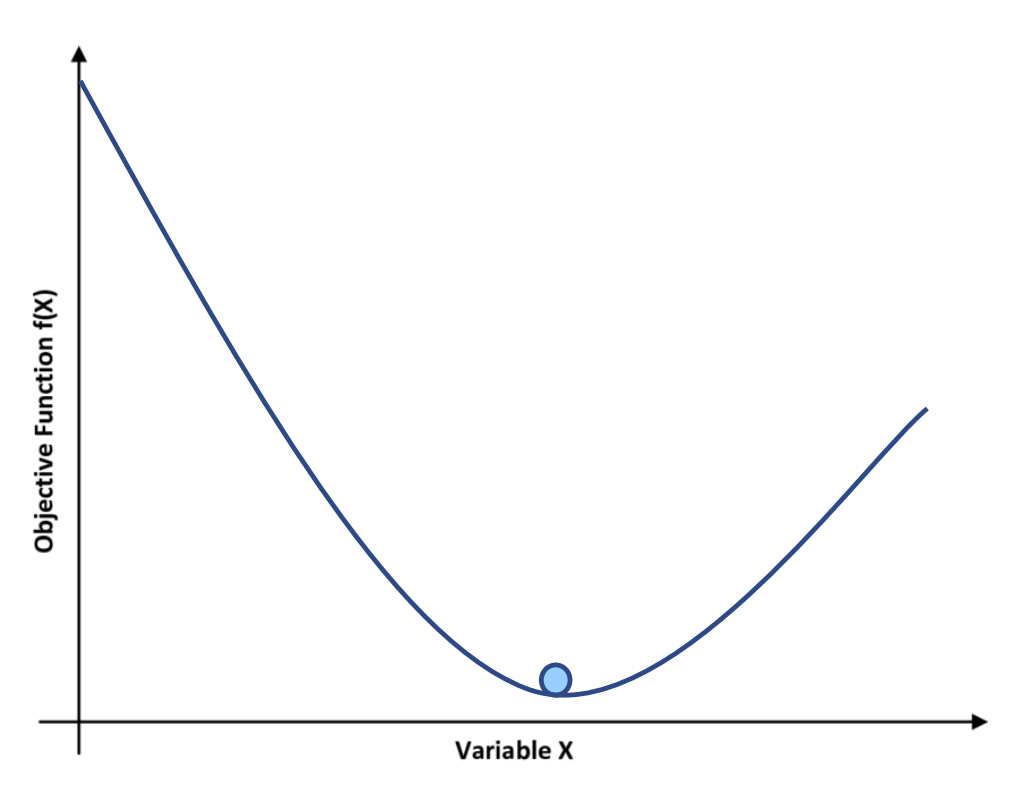
\includegraphics[width=0.7\textwidth]{images/simple_function.png}
    \caption{Hàm năng lượng khởi tạo là một hàm năng lượng đơn giản để đảm bảo trạng thái lượng tử ở mức năng lượng thấp nhất (ground state).}
    \label{fig:Đồ thị hàm số một hàm đơn giản}
\end{figure}

Quá trình ủ bao gồm việc sửa đổi từ từ hàm mục tiêu để thay đổi dần hình dạng của nó. Quá trình này kéo dài cho đến khi hàm mục tiêu ban đầu trở nên tương đương với hàm mục tiêu mà thực sự muốn tối ưu hóa. 
Nếu quá trình ủ diễn ra đủ chậm thì Định lý Đoạn nhiệt đảm bảo với chúng ta rằng trong tất cả các giai đoạn biến đổi của hàm mục tiêu, điểm cực tiểu toàn cục đã thích ứng với hình dạng của hàm. (Hình~\ref{fig:Biến đổi hàm mục tiêu})

\begin{figure}[h!]
    \centering
    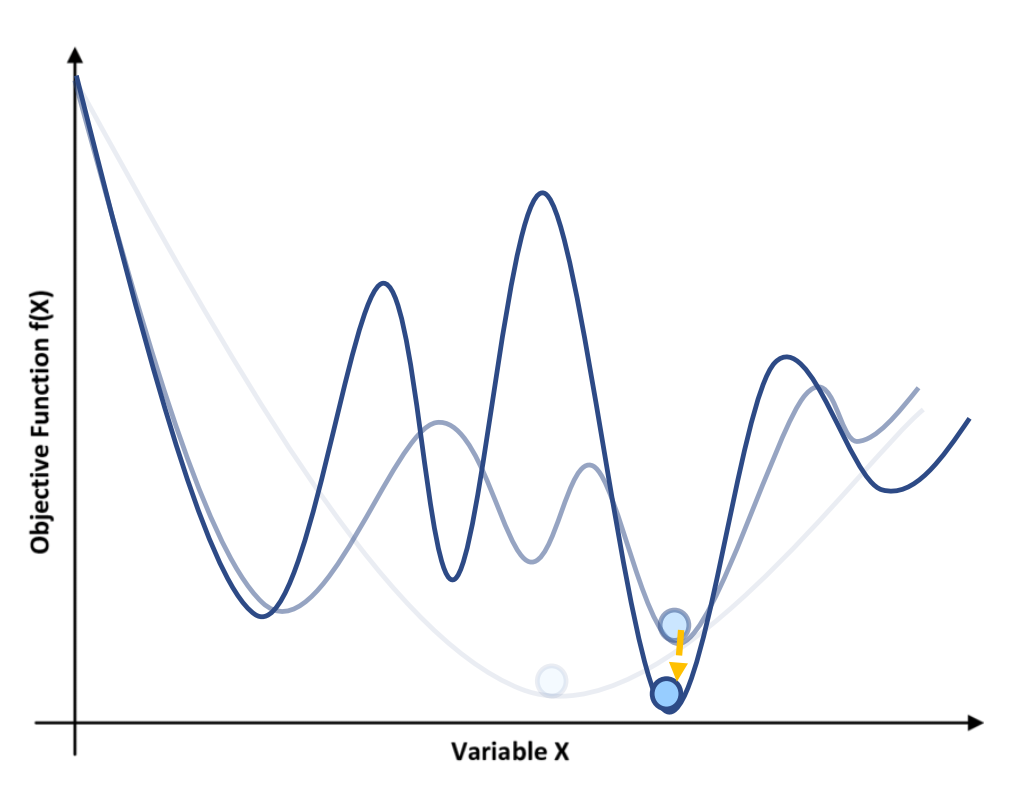
\includegraphics[width=0.7\textwidth]{images/QA.png}
    \caption{Quá trình ủ lượng tử từ từ diễn ra đủ chậm thì trạng thái lượng tử vẫn giữ ở mức năng lượng thấp nhất}
    \label{fig:Biến đổi hàm mục tiêu}
\end{figure}

Để hiểu cách tương tác với máy ủ lượng tử, chúng ta cần các khái niệm sau:

\begin{itemize}
  \item Hàm mục tiêu
  \item Bài toán tối ưu hóa nhị phân không ràng buộc bậc hai (QUBO)
  \item Đồ thị và nhúng
  
\end{itemize}

\subsection{Hàm mục tiêu và ràng buộc}


Để biểu diễn một bài toán giải quyết nó thông qua quá trình ủ lượng tử, trước hết chúng ta cần một hàm mục tiêu. Hàm mục tiêu là một biểu thức toán học của năng lượng của một hệ thống. Nói một cách đơn giản, nó đại diện cho hàm có giá trị tối thiểu mà bạn muốn tìm và năng lượng ở đây là hàm của các biến nhị phân đại diện cho hạt lượng tử của nó. (Hình~\ref{fig: Đồ thị năng lượng hàm mục tiêu})

\begin{figure}[H]
    \centering
    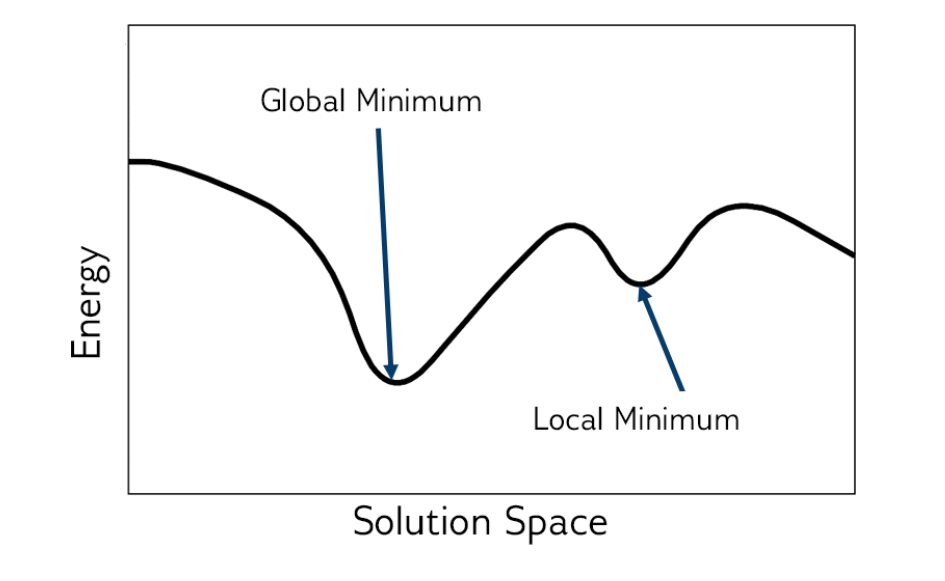
\includegraphics[width=0.7\textwidth]{images/objective_function.png}
    \caption{Nếu quá trình ủ diễn ra nhanh hoặc do nhiễu của thiết bị thì xác suất chính của trạng thái lượng tử rơi vào cực trị địa phương, làm bài toán không tìm được lời giải tối ưu.}
    \label{fig: Đồ thị năng lượng hàm mục tiêu}
\end{figure}

Trong hầu hết bài toán, năng lượng càng thấp thì lời giải càng tốt. Đôi khi bất kỳ trạng thái năng lượng tối thiểu cục bộ nào cũng là một lời giải có thể chấp nhận được cho bài toán ban đầu; đối với các bài toán khác chỉ có lời giải tối ưu mới được chấp nhận.

\subsection{Bài toán tối ưu hóa nhị phân không ràng buộc bậc hai (QUBO)}
Bài toán tối ưu hóa nhị phân không ràng buộc bậc hai là bài toán nổi tiếng trong lĩnh vực tối ưu hóa tổ hợp.
Bài toán QUBO được xác định bằng ma trận đường chéo Q, là một ma trận tam giác trên N x N  có trọng số thực và x, một vectơ của các biến nhị phân.\\
Hàm mục tiêu được biểu diễn dưới dạng bài toán QUBO như sau:
\[\text{E}_{qubo}(a_i, b_{i,j}; q_i) = \sum_{i} a_i q_i + \sum_{i<j} b_{i,j} q_i q_j.
\]
Trong đó các số hạng đường chéo của ma trận Q đóng vai trò là hệ số tuyến tính, còn các phần tử khác 0 là hệ số bậc hai
\[\min_{{x} \in {\{0,1\}^n}} {x}^{T} {Q}{x}.
\]

Hàm phạt là một đại lượng bổ sung cho bài toán tối ưu hóa ban đầu, đại lượng này phải được tối ưu hóa để toàn bộ bài toán được tối ưu hóa.

\subsection{Đồ thị và nhúng}
Về mặt toán học, đồ thị vô hướng được định nghĩa là một tập hợp các đỉnh
(V) và tập các cạnh (E)
Mỗi đỉnh và mỗi cạnh có thể được đánh trọng số.
Bằng cách này, có thể thiết lập sự tương ứng một-một giữa đồ thị có trọng số và hàm QUBO.

Cốt lõi của máy ủ lượng tử được biểu thị bằng đồ thị: trong hình~\ref{fig: Pegasus_qubits}, chúng ta có thể quan sát ô đơn vị của cấu trúc liên kết Chimera, đó là cấu trúc liên kết của một trong các mô hình D-Wave.
Điều này có nghĩa là để giải bài toán QUBO, cần phải ánh xạ bài toán lên đồ thị của máy ủ lượng tử đã chọn. Thủ tục này gọi là nhúng.

\begin{figure}[H]
    \centering
    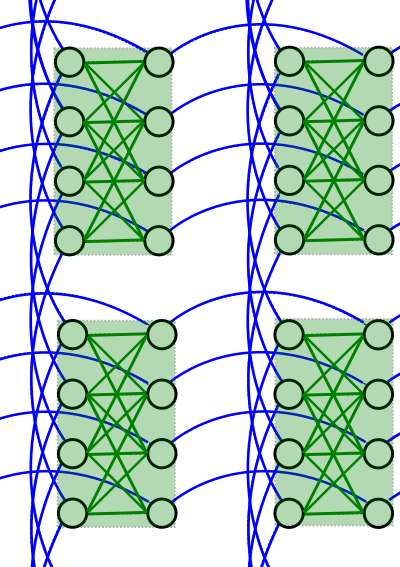
\includegraphics[width=0.5\textwidth]{images/Chimera_2x2_unit_cells.png}
    \caption{Hai ô đơn vị của biểu đồ Chimera. Hạt lượng tử được sắp xếp thành 4 ô đơn vị (hình vuông màu xanh lục mờ) được kết nối với nhau bằng bộ ghép bên ngoài (đường màu xanh lam) \cite{Topologies}}
    \label{fig: Pegasus_qubits}
\end{figure}



% Các biến thể của bài toán